%!TEX root = ../dissertation.tex

\chapter{The LHCb Experiment}
\label{chp:experiment}
%\epigraph{Las dein Auge am Rohr, Sagredo. Was du siehst, ist, dass es keinen Unterschied zwischen Himmel und Erde gibt. Heute ist der 10. Januar 1610. Die Menschheit trägt in ihr Journal ein: Himmel abgeschafft.}{Bertolt Brecht, Leben des Galilei}

%\epigraph{Keep your eye at the telescope, Sagredo. What you see means that there is no difference between Heaven and Earth. Today is the 10th January 1610. Mankind will write in its journal: Heaven abolished}{Bertolt Brecht, \textit{Life of Galileo}}
\section{The Large Hadron Collider}
The Large Hadron Collider (LHC) is a 27 km long circular accelerator, positioned at CERN, the European Organization for Nuclear Research, on the Swiss-French border. Constructed approximately 100  metres underground, LHC is the world's largest and most powerful particle accelerator, capable of accelerating protons and heavy ions to the unprecedented energy of \SI{14}{\tera\eV}.

Before reaching the LHC, protons are extracted from hydrogen gas and subjected to a series of acceleration stages, depicted in Figure~\ref{fig:LHC_scheme}~\cite{Lopienska:2800984}. Initially, LINAC4 accelerates hydrogen ions~(H$^-$) to \SI{160}{\mega\eV}. These ions then enter the Proton Synchrotron Booster, which strips the electrons, leaving only the protons and accelerating them to \SI{1.4}{\giga\eV}. From there, the protons are injected into the Proton Synchrotron (PS), reaching \SI{26}{\giga\eV}, and then into the Super Proton Synchrotron (SPS), which boosts them to \SI{450}{\giga\eV}. The SPS then injects the beams of protons into the LHC, where they are accelerated to their final energies by radio-frequency cavities and guided through the accelerator by superconducting magnets.
\begin{figure}[ht]
    \centering
    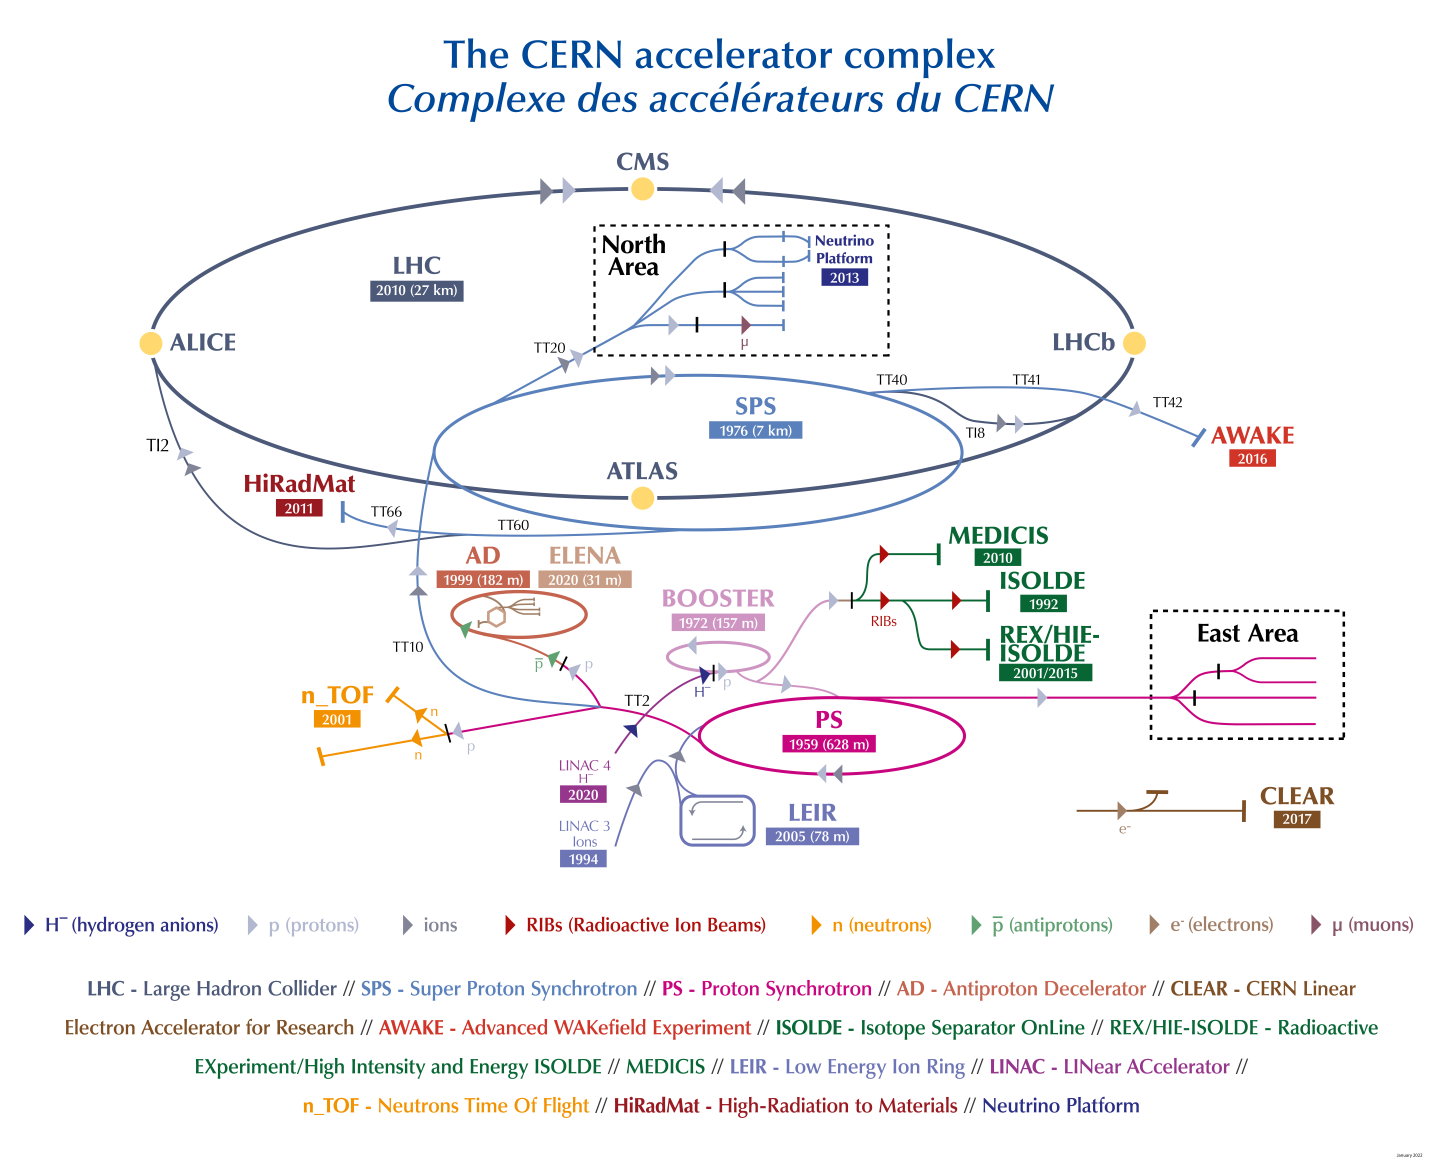
\includegraphics[width=\textwidth]{figures/CCC-v2022-large.png}
    \caption{The CERN accelerator complex is a succession of machines, where each machine accelerates a beam of particles to a given energy before injecting the beam into the next one in the chain. This next machine brings the beam to an even higher energy and so on. The LHC is the last element of this chain, in which the beams reach their highest energies.}
    \label{fig:LHC_scheme}
\end{figure}
The accelerator contains over 1200 superconducting dipole magnets, each about 15 metres long, to bend the beams, while 392 quadrupole magnets maintain beam focus. To ensure optimal performance, these magnets are cooled to \SI{1.9}{\kelvin} using superfluid helium. The LHC operates with two beams of protons or heavy ions circulating in opposite directions in separate beam pipes. Proton beams within the LHC are divided into 2808 bunches, each containing approximately $10^{11}$ protons. These bunches are time-spaced by multiples of \SI{25}{\nano\second}, resulting in a bunch-crossing frequency of up to \SI{40}{\mega\hertz}, with an average bunch-crossing rate of approximately \SI{30}{\mega\hertz}. 
The LHC started operating in 2008 and collided the first beams at an energy of $\sqrt{s}=\SI{450}{\giga\eV}$ in 2009 and has undergone significant upgrades during its operation. The start of the physics research programme was marked by the beginning of Run~1 in 2010 with collisions at a center-of-mass energy of  $\sqrt{s}=\SI{7}{\tera\eV}$, subsequently upgrading this energy to \SI{8}{\tera\eV} in 2012. After LS1, in 2015 the LHC began Run~2 colliding beams at a ground breaking energy of  $\sqrt{s}=\SI{13}{\tera\eV}$. During Run 3, begun in 2022, the LHC aims at reaching its peak design parameters, including a center-of-mass energy of $\sqrt{s}=\SI{14}{\tera\eV}$ and an instantaneous luminosity of $\mathcal{L}\approx\SI{2e34}{\per\centi\meter\squared\per\second}$.

The high-energy beams collide at four designated points along the LHC ring, which house the major experiments: ATLAS, CMS, ALICE, and LHCb.
The experiments at the LHC serve different purposes. ATLAS and CMS are general-purpose detectors focusing on high-luminosity collisions to study a wide range of physics phenomena, including the search for new particles, extra dimensions, and dark matter. ALICE, a heavy-ion experiment, explores the quark-gluon plasma, a state of matter present shortly after the Big Bang. LHCb specializes in heavy-quark physics and operates at mid-range luminosity, focusing on flavor physics and $\mathcal{CP}$ violation studies.

\section{The LHCb Detector}

The LHCb detector, depicted in Figure~\ref{fig:lhcb-detector}, is a single-arm forward spectrometer, with a pseudorapidity coverage of 2 to 5. This unique design allows it to study particles containing heavy quarks, primarily bottom ($b$) and charm ($c$), which are typically produced at high pseudorapidity during proton-proton ($pp$) collisions. The LHCb underwent a significant upgrade during LS$2$ to accommodate increased luminosity and handle the elevated event rate associated with the upgraded LHC.
\begin{figure}[h]
    \centering
    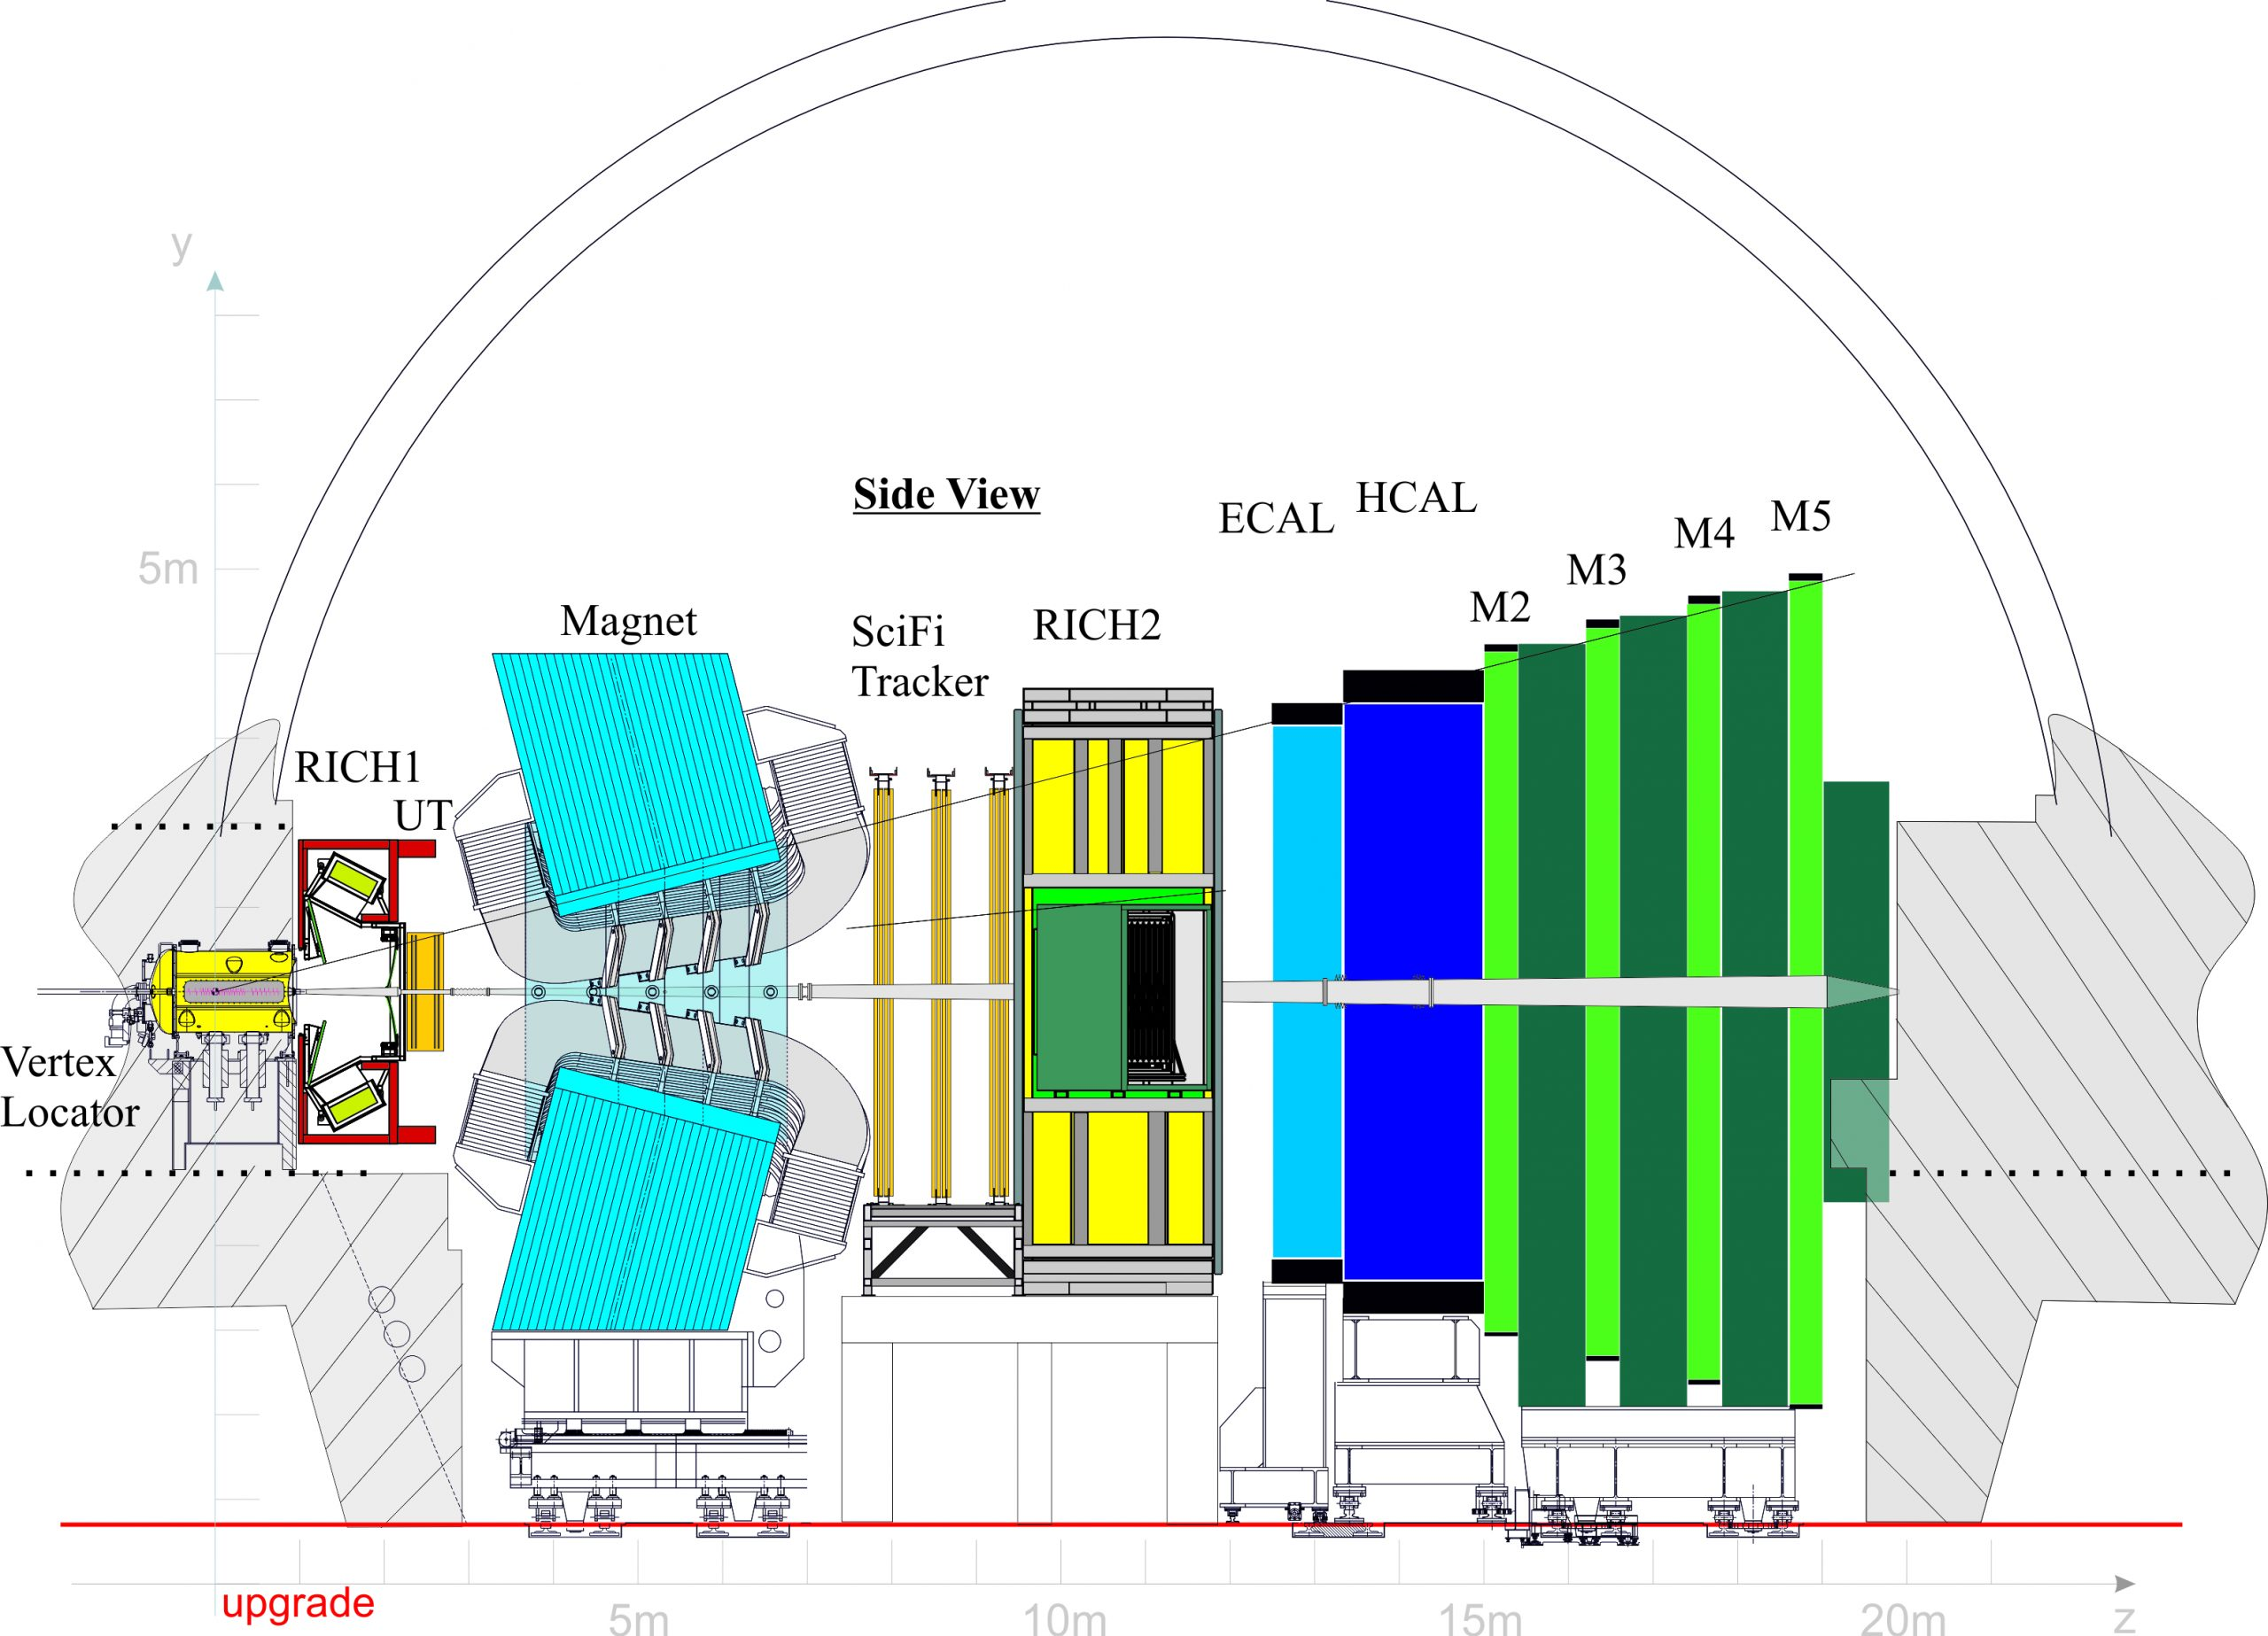
\includegraphics[width=\textwidth]{figures/UT-upgrade-detector-scaled.jpeg}
    \caption{Layout of LHCb-Upgrade I detector, side-view from the center of LHC ring.}
    \label{fig:lhcb-detector}
\end{figure}
With the upgrade, LHCb will operate at an average bunch-crossing rate of approximately \SI{30}{\mega\hertz}, with an expected instantaneous luminosity of about \SI{2e33}{\per\centi\meter\squared\per\second}. The average number of pp collisions per bunch-crossing  is anticipated to be around $\mu=5.5$. During Run-3 and Run-4, the experiment aims to collect at least \SI{50}{\per\femto\barn} of data, enabling unprecedented precision in measurements within the flavor sector of the Standard Model.

Key upgrades include:
\begin{itemize}
\item \textbf{Tracking System}: The tracking system has been renewed, with a new silicon pixel detector, the Vertex Locator (VELO), which measures primary and secondary vertex positions with high precision. Additionally, a new silicon strips upstream tracker (UT) and a scintillating fibers tracker (SciFi) for track fitting were installed.

\item \textbf{Trigger System}: The trigger system has been completely overhauled. In Run~1 and Run~2, LHCb used a Level-zero (L$0$) hardware trigger, which reduced the data acquisition rate from \SI{40}{\mega\hertz} to \SI{1.1}{\mega\hertz}, based on information from the Calorimeter system and Muon stations. This system was removed after Run~2 in favour of a more flexible trigger. The upgraded trigger system now reconstructs the entire event in real-time, enabling high selection efficiency for a wide range of events. The upgraded data acquisition system allows LHCb to process all the data from each collision in real time, allowing to select which events to save based on fully reconstructed decay trees. This system plays a crucial role in ensuring the experiment ability to handle increased data flow and maintain high selection efficiency.
\end{itemize}
In the following sections an overview of each subdetector will be given.

\subsection[VErtex LOcator]{VErtex LOcator $\bigl($VELO$\bigr)$}
The Vertex Locator (VELO)~\cite{Bediaga:2013tje} is a silicon pixel detector designed to reconstruct primary and secondary decay vertices. In general, a pixel detector operates by detecting charged particles as they traverse a matrix of discrete sensing elements (pixels). When a charged particle hits a pixel, it generates an electrical signal, which is then processed to determine the particle's position and other properties.  
%The spacial resolution of the VELO needs to be better than the typical length of $b$ and $c$ hadrons, ranging from $100$ to \SI{500}{\micro\meter}.  

The VELO consists of 26 stations, which are pairs of retractable modules placed within the LHC vacuum pipe, in order to be as close as possible to the beamline. 
A brief schematics of the geometry is reported in Figure~\ref{fig:velo-geometry}~\cite{LHCbVelo:2019flq}. Figure~\ref{fig_velo-xy} shows the behaviour of the two retractable modules in the fully closed (left) and fully open (right) configuration. In its fully closed configuration, the innermost VELO sensor is just \SI{5.1}{\milli\meter} from the nominal interaction point, making it the closest detector to the beamline in any HEP experiment at CERN. During beam ramping, the modules are moved to a safer position of approximately \SI{3}{\centi\meter} from the beamline, in order to prevent damage from instabilities of the high-energy beams in the LHC.

A top view of the 26 stations is visible in Figure~\ref{fig_velo-side}, together with the illustrations of the $z$-extent of the luminous region at $y=0$ and the nominal LHCb acceptance given by the pseudorapidity $\eta$. 

\begin{figure}
    \centering
    \begin{subfigure}{0.48\textwidth}
    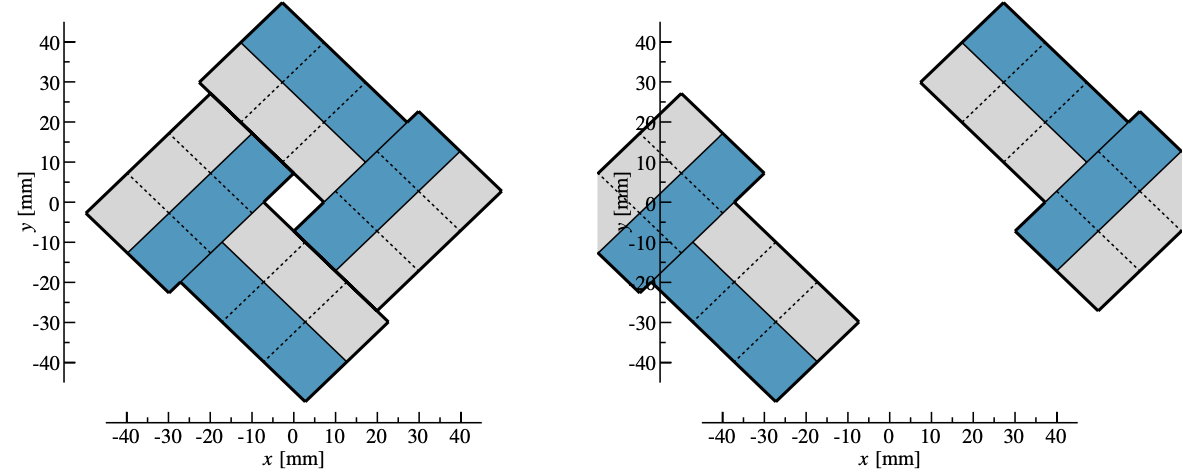
\includegraphics[width=\linewidth]{figures/aperture.png}
    \caption{View of a station in the x-y plane. The two modules, VELO A on the right and VELO C on the left, can be opened and closed}\label{fig_velo-xy}
    \end{subfigure}
    \begin{subfigure}{0.48\textwidth}
    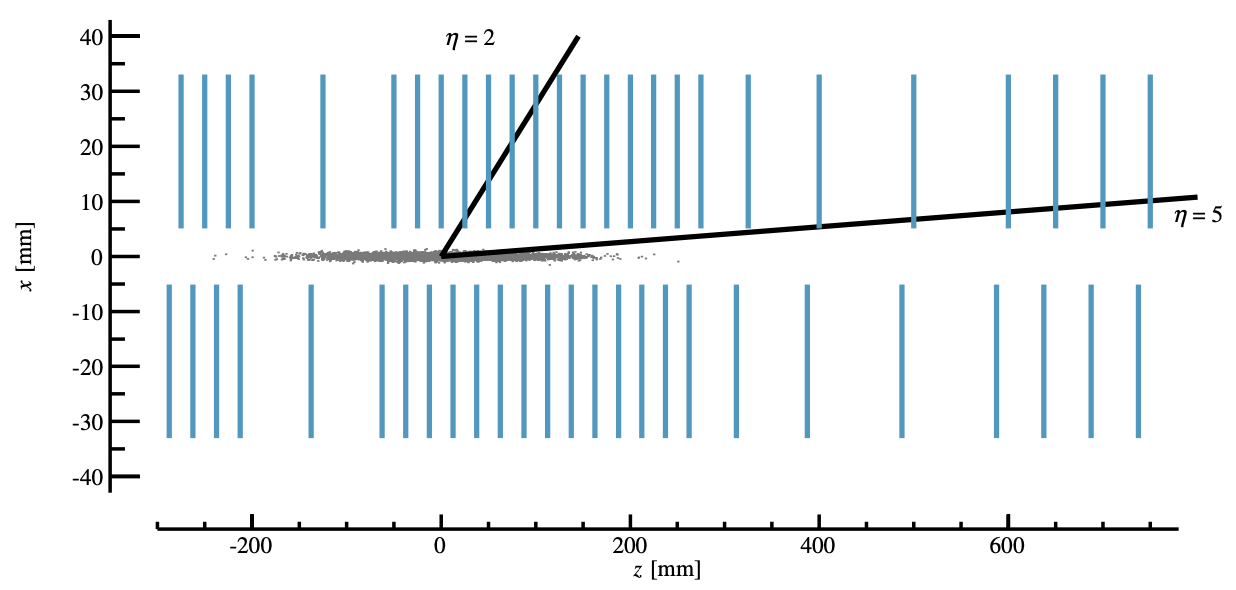
\includegraphics[width=\linewidth]{figures/above_view.png}
    \caption{Top view of all the 52 modules in the x-z plane}\label{fig_velo-side}
    \end{subfigure}
    \caption{Two different schematics of the geometry of the VELO. Figure \ref{fig_velo-xy} shows a view of the plane perpendicular to the beam pipe. The possible aperture of the two modules is also displayed. Figure \ref{fig_velo-side} shows a view from the side, where we appreciate each side section of the VELO.}
    \label{fig:velo-geometry}
\end{figure}

Each module contains two tiles, and each tile has two sensors. Each sensor consists of 768 × 256 pixels, with a thickness of \SI{200}{\micro\meter}. 
The VELO sensors are read out by VeloPix ASICs, each featuring a 256 × 256 matrix of active silicon pixels with dimensions of \SI{55}{\micro\meter} × \SI{55}{\micro\meter}. The entire VELO system contains over 40 million pixels. The raw hit resolution varies between $9$ and \SI{15}{\micro\meter}, depending on the angle of the incoming particle. To maintain detection efficiency and account for highly inclined tracks, a 2-pixel wide overlap between sensors within the same tile is implemented. This overlap ensures no gaps in the detection coverage.
%designed to operate at high frequencies (up to \SI{40}{\mega\hertz}) and to withstand intense radiation levels.

At the trigger level, the VELO detects tracks with high impact parameters, which are indicative of heavy-flavored particle decays, helping reducing the minimum bias rate by providing initial track information. Offline, high-resolution vertex reconstruction is key to studying heavy-meson oscillations and $\mathcal{CP}$-dependent time asymmetries.
\subsection{Upstream Tracker}
The UT is a micro-strip silicon detector made of four layers~\cite{LHCb:2014uqj}. It replaced the former TT detector, retired to due irradiation. Each UT sensor is composed of \SI{250}{\micro\meter} thick silicon and a \SI{10}{\micro\meter} metalization layer. The segmentation is finer than the TT, with near-beam sensor pitch of \SI{95}{\micro\meter} and dimension of $98$×\SI{49}{\milli\meter}, against the TT sensor pitch of \SI{183}{\micro\meter}. In Figure~\ref{fig:UT} a view of the detector is shown~\cite{ut}. 
The UT is a core part of the LHCb physics case, being required to constrain important decays such as $K_S \rightarrow\pi\pi$ that happen beyond the VELO acceptance. The UT also boosts the momentum resolution and helps identify ghost tracks.

\begin{figure}
    \centering
    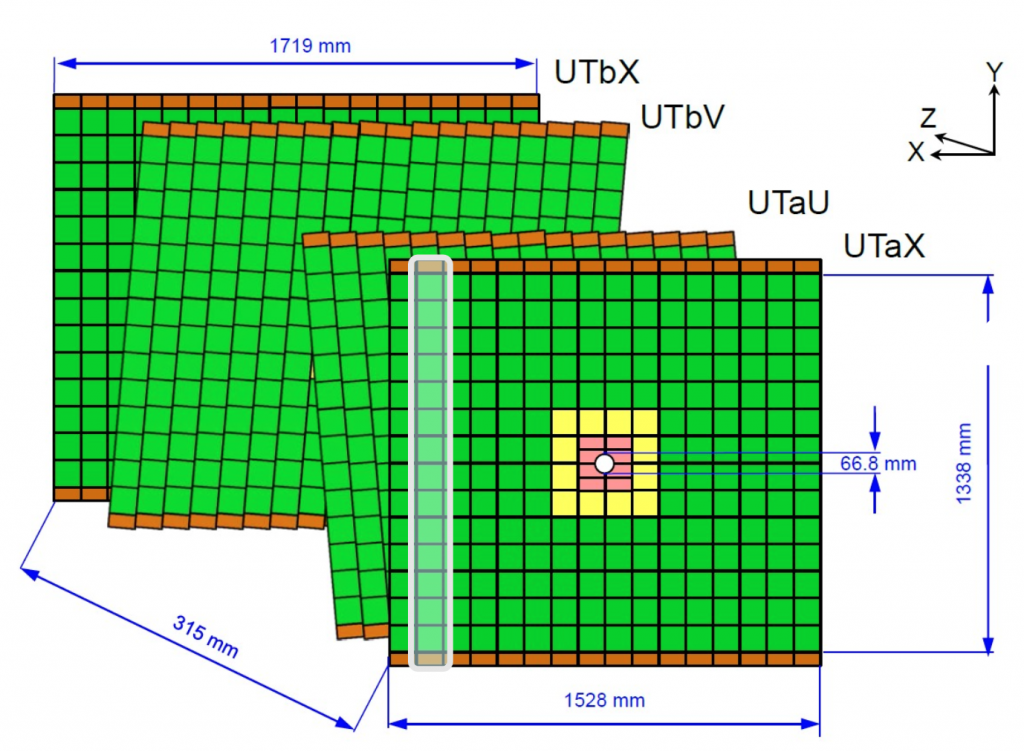
\includegraphics[width=0.7\textwidth]{figures/UT.png}
    \caption{Overview of the UT schematic layout}
    \label{fig:UT}
\end{figure}

\subsection{Magnet}
LHCb exploits the forward region of proton collisions and requires a dipole field with a free aperture of \SI{\pm300}{\milli\radian} horizontally and \SI{\pm250}{\milli\radian} vertically. In order to achieve this, LHCb has a magnet~\cite{LHCb:2000xej} consisting of two coils, both weighing 27 tonnes, mounted inside a 1450 tonne steel frame. Each coil is constructed from 10 layers, wound from almost 3000 metres of aluminium cable. A schematics of the magnet is depicted in Figure \ref{fig:magnet}.
Tracking detectors in the magnetic field have to provide momentum measurement for charged particles with a precision of about 0.4\% for momenta up to $200$ GeV/$c$. This demands an integrated field of \SI{4}{\tesla\meter} for tracks originating near the primary interaction point.
 The lateral aperture of the magnet is defined by the longitudinal extension of the detectors, placed upstream of the magnet. The two coils are each \SI{7.5}{\meter} long, \SI{4.6}{\meter} wide and \SI{2.5}{\meter} high.
\begin{figure}
    \centering
    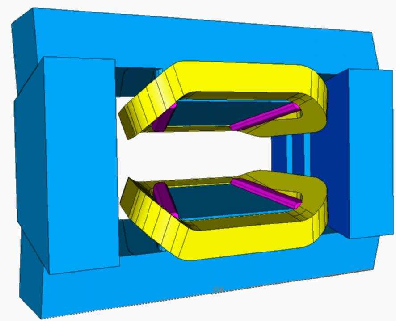
\includegraphics[width=0.5\textwidth]{figures/lhcb-magnet.png}
    \caption{A schematic of the LHCb magnet (yellow) with the yoke (blue) supporting it}
    \label{fig:magnet}
\end{figure}
The LHCb magnet has a unique feature consisting into the possibility to reverse the polarity of the magnetic field (MagUp or MagDown). This allows a precise control of the charge asymmetries introduced by the detector. Particles hit preferentially one side of the detector, depending on their charges, generating potentially large detection asymmetries. If the data samples collected with the two different polarities have approximately equal size and if the operating conditions are stable enough, charge asymmetries are expected to cancel.

\subsection[Scintillating Fibre Tracker]{Scintillating Fibre Tracker$ \bigl($SciFi$\bigr)$}
The Scintillating Fibres tracker (SciFi)~\cite{scifi} is another tracker subdetector, that provides enhanced pattern recognition, momentum estimation, and overall tracking efficiency.
The SciFi is located downstream of the dipole magnet and consists of three tracking stations: T$1$, T$2$, and T$3$. Each station comprises four detection planes, arranged to measure coordinates in a cross-pattern, with the orientation of the fiber strips at angles of $\SI{0}{\degree}$, $\SI{+5}{\degree}$ and $\SI{-5}{\degree}$ relative to the vertical axis. These layers are made up of 12 modules, measuring \SI{5}{\meter} by \SI{52}{\centi\meter}, with the innermost modules containing six fiber layers, and the others containing five, due to lower radiation levels. This configuration offers high resolution in the bending plane of the magnetic field and supports efficient pattern recognition for charged particles.

The structural design features vertical staves in the first and last detection planes, while the central two have tilted staves, creating a balanced configuration that enhances detection capabilities and minimizes gaps in coverage. Each detector module is constructed with $2.5$-meter-long scintillating fibers, \SI{250}{\micro\meter} in diameter. 
A scheme of the detector geometry is reported in Figure \ref{fig:scifi}.
Scintillating fibers are made from a polymer core with 1\% by weight of fluorescent dye added to enhance scintillation. The fibers generate optical photons upon interaction with ionizing radiation. This process involves depositing energy in the polymer core, which excites the material. Due to the inherent limitations of the base polymer in terms of light yield and relaxation time, the addition of the fluorescent dye improves efficiency by matching energy-level structures to enhance photon production.

The SciFi uses Silicon Photomultipliers (SiPMs) to read the optical photons. These SiPMs are contained in read-out boxes located at the top and bottom of each detection plane, ensuring efficient collection and processing of the scintillation signals. The SiPMs offer high gain, fast response, and compactness, allowing them to be integrated into the compact design of the SciFi system.

The SciFi is designed for a high hit efficiency, with simulated performance indicating a hit efficiency of over 97\% at the end of its operational lifetime. The raw hit resolution is expected to be approximately \SI{42}{\micro\meter}, providing precise measurements of charged particle trajectories.

\begin{figure}
    \centering
    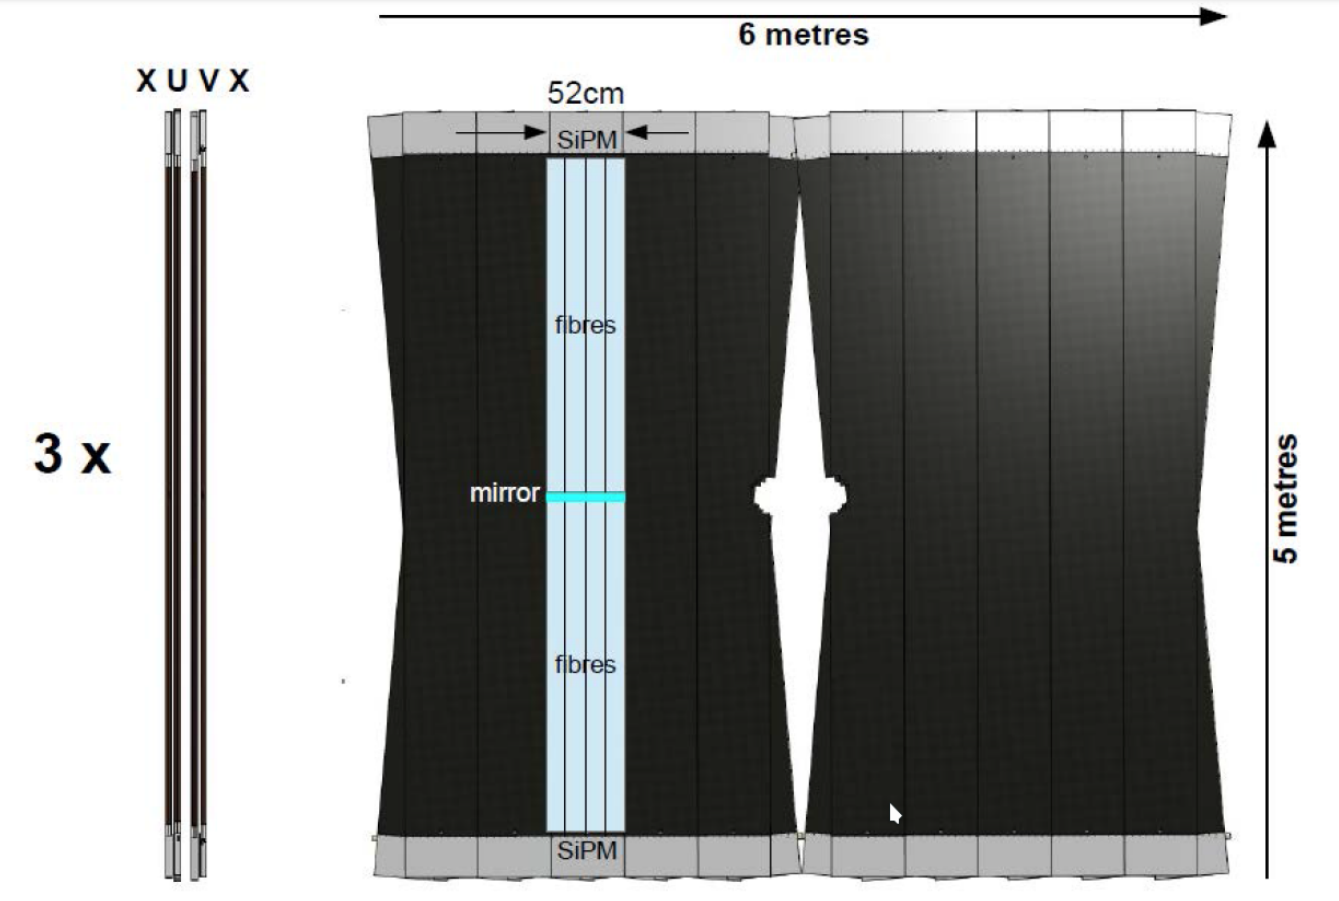
\includegraphics[width=0.7\textwidth]{figures/scifi.png}
    \caption{A schematics of the SciFi}
    \label{fig:scifi}
\end{figure}


\subsection{RICH}
At LHCb there are two Ring Imaging Cherenkov (RICH) detectors, RICH1 and RICH2, that enable particle identification~\cite{LHCb:2013urp} across a broad momentum range, from $1$ to $100$ GeV/c~\cite{Adinolfi_2013}.

Cherenkov radiation occurs when charged particles travel through a dielectric medium at speeds exceeding the local speed of light (superluminal speed). The angle at which Cherenkov radiation is emitted (Cherenkov angle) is directly related to the refractive index of the medium and the velocity of the particle. Given this relation, the Cherenkov angle $\theta_c$ can be used to infer the mass of a particle when its momentum is known:

\begin{equation}
    \cos\theta_c=\frac{1}{\beta n} = \frac{1}{n}\sqrt{1+\biggl(\frac{m}{p}\biggr)^2}
\end{equation}

where $\beta$ is the speed of the particle relative to the speed of light in natural units ($c=1$), $n$ is the refractive index of the medium, $m$ is the particle mass, and $p$ is its momentum.
This principle allows for the identification of different particles based on the Cherenkov angle. The RICH system uses this concept to separate charged hadrons over a momentum range of $1-100$ GeV/c, essential for studying hadronic final states and central to LHCb's physics goals, including precise measurements of $\mathcal{CP}$ violation and rare decays of b and c hadrons.

RICH$1$ is located between the VELO and the UT, upstream of the spectrometer magnet. It uses two radiators, aerogel (with refractive index $n=1.03$) and C4F10 (with refractive index $n=1.0014$), allowing discrimination of particles over a momentum range of $1-60$ GeV/c. RICH$1$ covers an angular acceptance of $25-300$ mrad.

RICH$2$ is downstream of the spectrometer magnet, after the last T-station, covering an angular acceptance from $15$ to $120$ mrad (non-bending plane) and $15$ to $100$ mrad (bending plane). It uses CF4 (with refractive index $n=1.0005$) as the radiator, allowing discrimination of particles with momentum ranging from $15$ to $\geq100$ GeV/c. The $\pi-K$ separation in RICH$2$ is approximately 90\% efficient for momenta up to $30$ GeV/c.

The RICH detectors use spherical mirrors to focus Cherenkov light, with secondary flat mirrors to guide the photons onto Hybrid Photon Detectors (HPDs). These HPDs are sensitive to photons in the $200-600$ nm wavelength range, and they are placed outside the detector acceptance, reducing material costs and protecting them from the spectrometer's magnetic field.

Arrays of multi-anode photomultiplier tubes (MaPMTs) are used to detect individual Cherenkov photons, with RICH$1$ having a total detection area of $\SI{1.6}{\squared\meter}$ and RICH$2$ having a detection area of $\SI{2.2}{\squared\meter}$. This arrangement ensures efficient collection and processing of Cherenkov light for particle identification.

\begin{figure}
    \centering
    \begin{subfigure}{0.48\textwidth}
    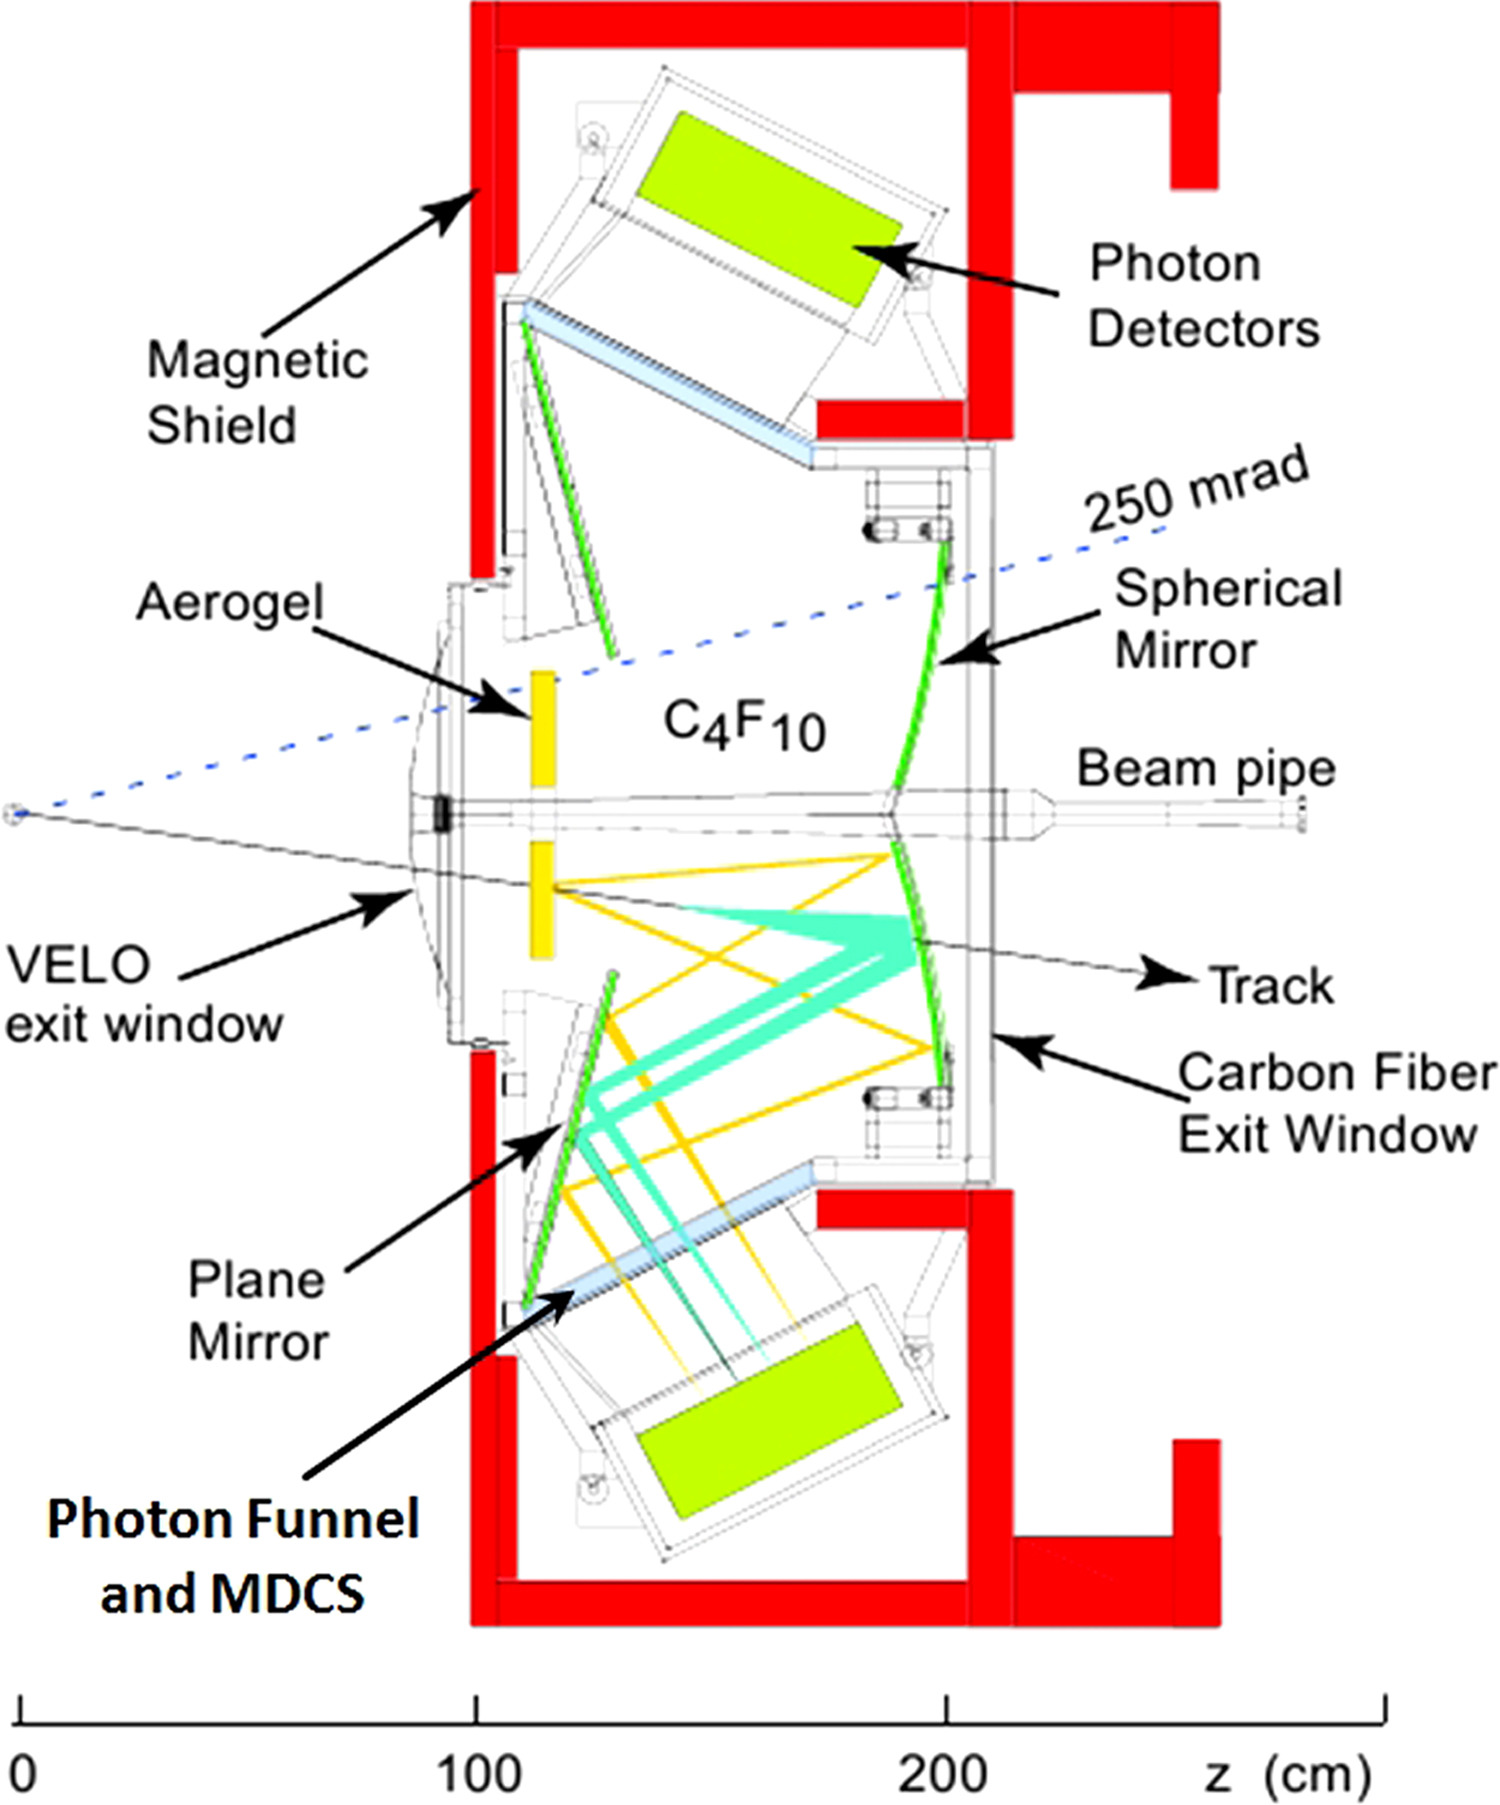
\includegraphics[width=\linewidth]{figures/rich1.jpg}
    \caption{RICH$1$}\label{RICH1}
    \end{subfigure}
    \hfill
    \begin{subfigure}{0.48\textwidth}
    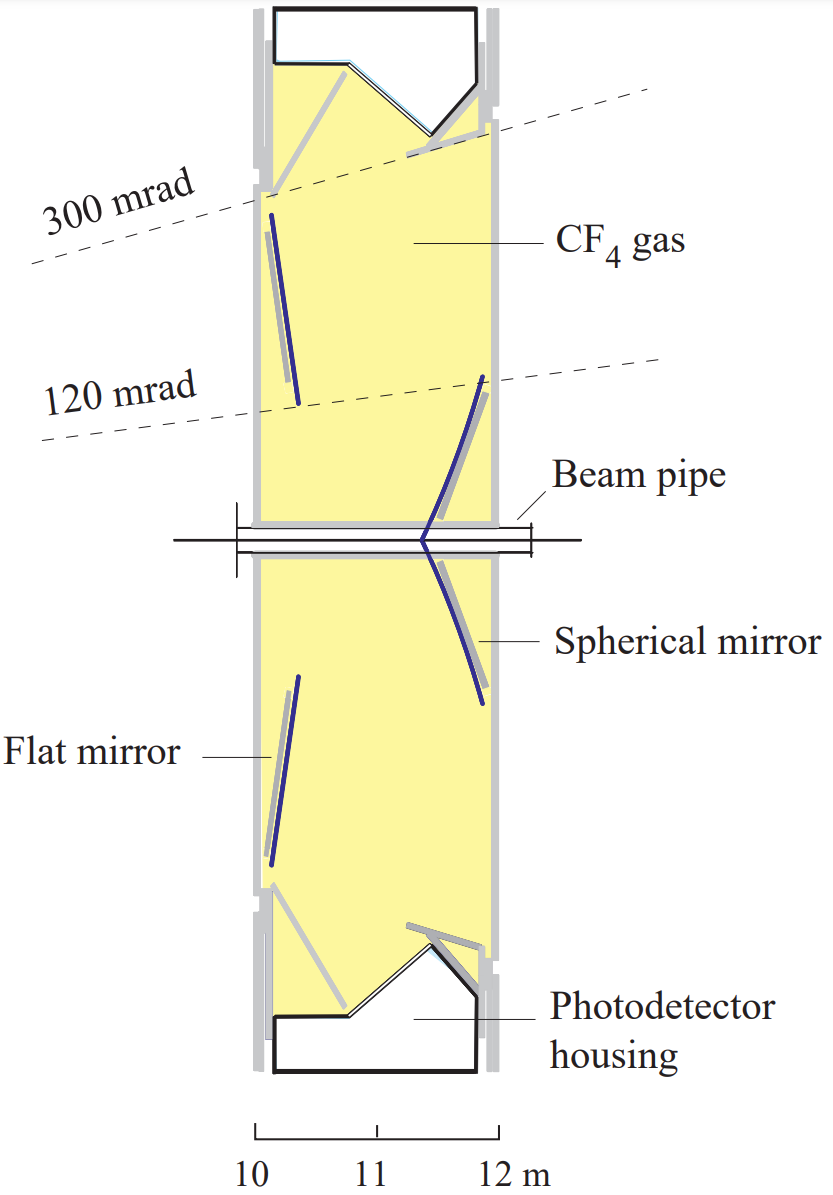
\includegraphics[width=0.78\linewidth]{figures/rich2.png}
    \caption{RICH$2$}\label{rich2}
    \end{subfigure}
    \caption{Schematics side view of the two RICH detectors.}
    \label{fig:rich}
\end{figure}

\subsection{Calorimeters}
\sloppy
The calorimeter system in the LHCb experiment~\cite{LHCb:2000vji} plays its role in identifying electrons, photons, and hadrons, providing a measurement of their energies and positions. The system comprises the Electromagnetic Calorimeter (ECAL) and an  Hadron Calorimeter (HCAL). Both of them are  placed between the first and the second muon stations, with an angular acceptance ranging from $25$ mrad to $300(250)$ mrad in the bending (non-bending) plane. 
The ECAL is responsible for measuring the energy and position of electrons and photons. It is built with shashlik calorimeter technology, consisting of alternating $4$~mm-thick polystyrene scintillating tiles and $2$ mm lead sheets. The scintillation light is collected using wavelength-shifting fibers and read out by individual photomultipliers (PMTs) mounted at the back of the tiles. The total thickness of the ECAL is 25 radiation lengths, providing sufficient thickness to contain most electromagnetic showers. The calorimeter structure is segmented into three zones depending on the radial distance from the beamline. The inner section has cells with a lateral dimension of $\SI{40.4}{\milli\meter}$, the middle section has cells with a $\SI{60.6}{\milli\meter}$ dimension, and the outer section comprises cells with a $\SI{121.2}{\milli\meter}$ dimension. The energy resolution for the ECAL is approximately 
 $\sigma_E/E$(GeV)=($8.5-9.5$).

\sloppy
The HCAL is responsible for measuring the energy and position of hadrons. It consists of $16$ mm-thick iron layers alternated with $\SI{2}{\milli\meter}$ scintillating fibers, with a total thickness corresponding to 5.6 nuclear interaction lengths. This design is constrained by the space available inside the LHCb cavern. The energy resolution for the HCAL is approximately $\sigma_E/E$(GeV)=($8.5-9.5$)/E(GeV)=$9$.

The lateral segmentation of both ECAL and HCAL is shown in Figure \ref{fig:cal_system}.
\begin{figure}
    \centering
    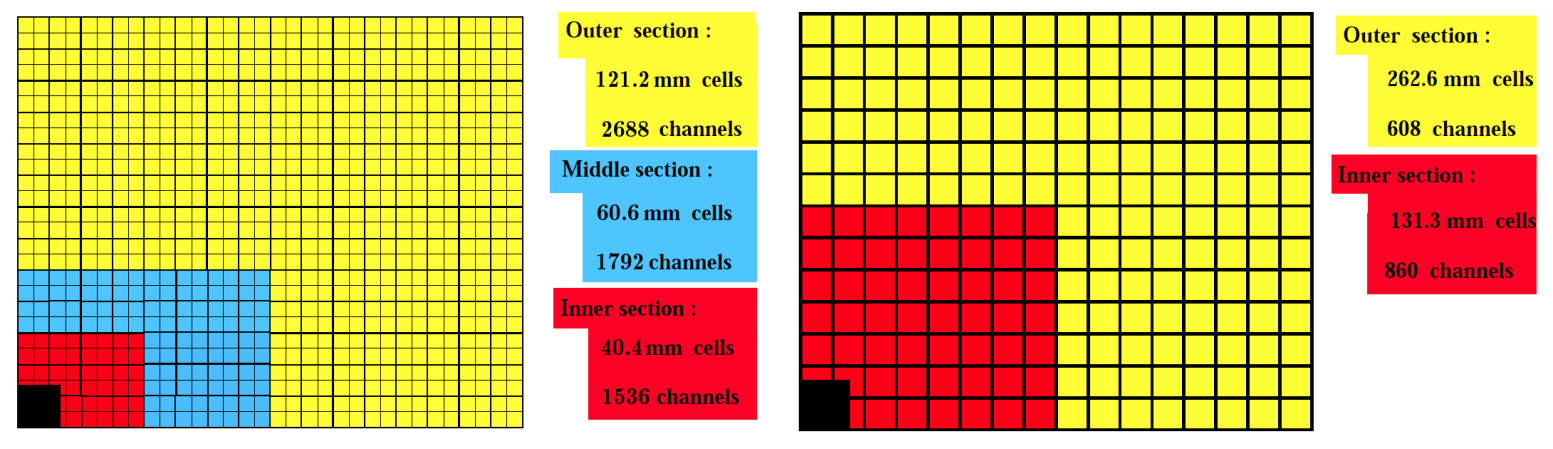
\includegraphics[width=\textwidth]{figures/CAL_system.png}
    \caption{Lateral segmentation of the ECAL (left) and the HCAL (right). One quarter of the detector front face is shown.}
    \label{fig:cal_system}
\end{figure}
\subsection{Muon Stations}

The muon detector system primary function is to identify and measure the transverse momentum of muons in order to reconstruct decay channels involving muons, which are vital for many LHCb physics studies.
The LHCb muon detector system~\cite{Alves_2013} consists of four stations (M$2$ to M$5$) placed downstream of the hadronic calorimeter and interleaved with thick iron walls that act as muon filters. In Run-1 and Run-2, there was an additional M$1$ station located in front of the calorimeters, used for transverse momentum measurement for the L$0$ trigger~\cite{muon_upgrade}. The system covers the angular acceptance from $20 (16)$ to $306 (258)$ mrad in the bending (non-bending) plane. Each station comprises two mechanically independent halves, called the A and C sides, which can be horizontally moved to access the beam pipe and detector chambers for installation and maintenance.
A scheme of the muon stations (including M1 no longer part of the detector) is depicted in Figure \ref{fig:muon}.
\begin{figure}
    \centering
    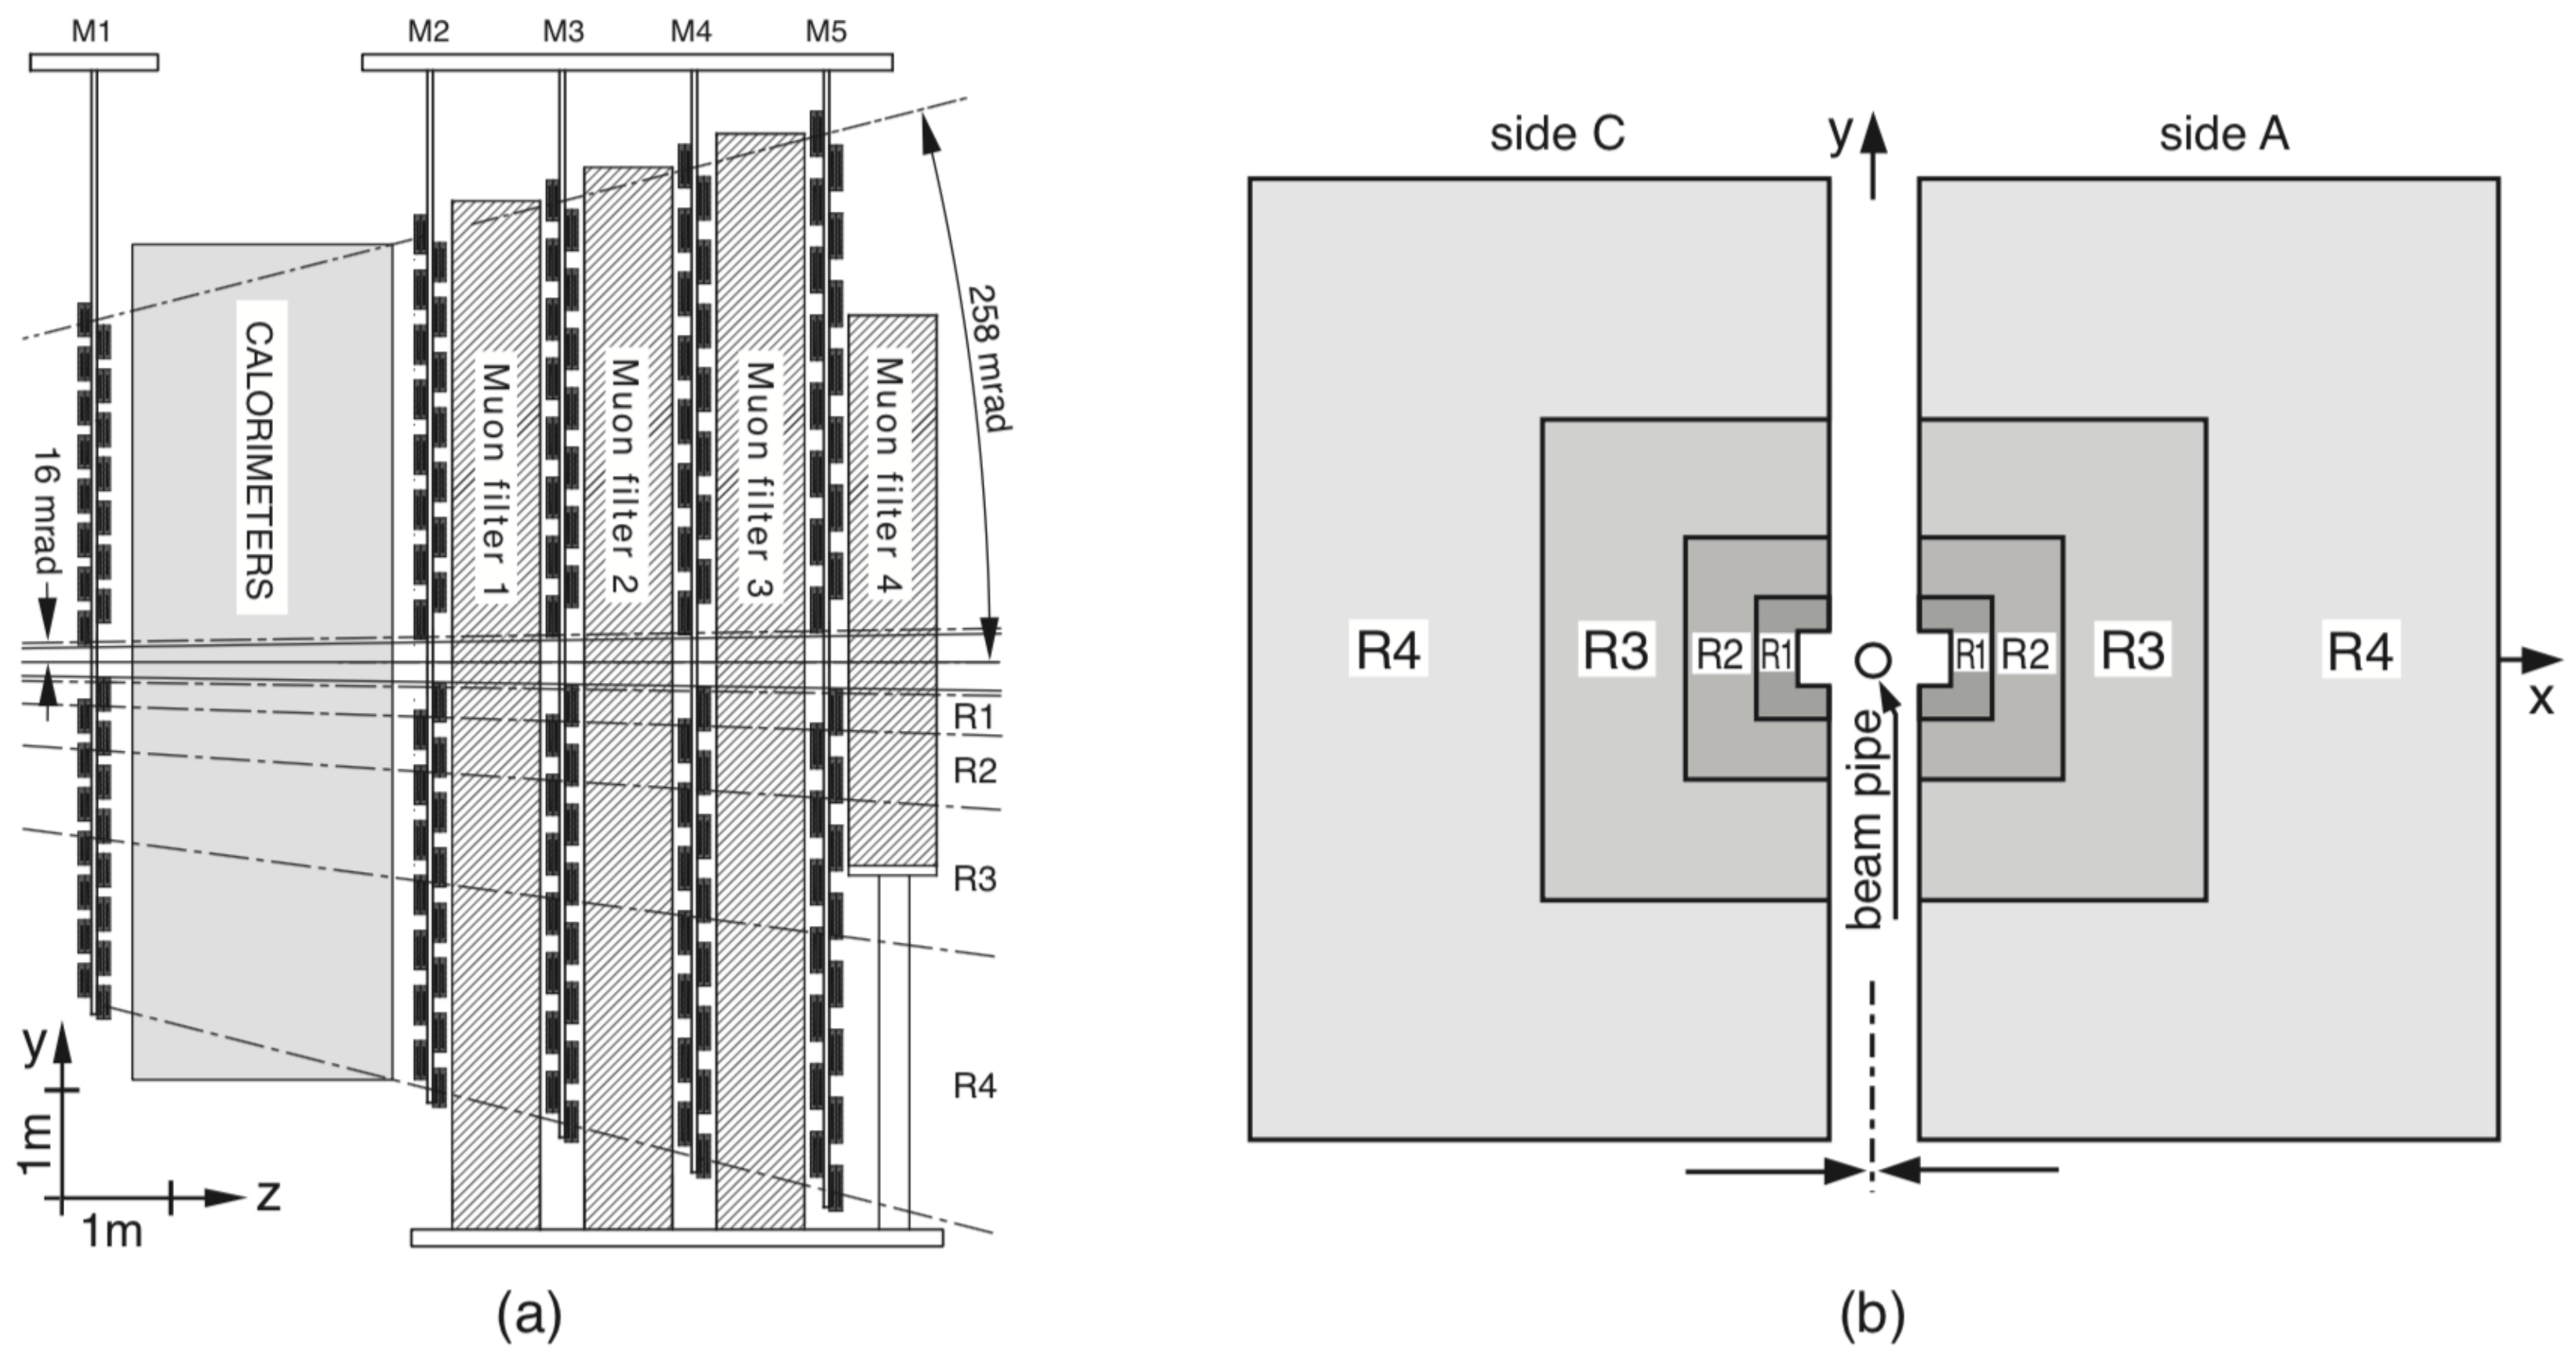
\includegraphics[width=\textwidth]{figures/muon.png}
    \caption{A scheme of the muon stations. M$1$ was removed during Upgrade 1.}
    \label{fig:muon}
\end{figure}
The stations are equipped with Multi-Wire Proportional Chambers (MWPCs) for muon detection. These chambers use a gas mixture of argon, carbon dioxide, and tetrafluoromethane (CF4) in varying proportions for optimal muon detection and signal collection. The iron absorbers between the stations add to the muon filtering capacity, ensuring that only muons with momentum greater than $6$ GeV/c can traverse the entire system.

Stations M$2$-M$3$ focus on transverse momentum measurements, while M$4$ and M$5$ serve to confirm if a particle has traversed the entire detector system. The system achieves a 95\% detection efficiency, providing robust muon identification. 

The unique feature of the LHCb muon detector system is its segmented structure, with each station divided into four regions (R$1$-R$4$), with cells scaling in the ratio 1:2:4:8 with distance from the beam axis. This segmentation allows the system to manage varying particle rates and optimize detection efficiency. Additionally, the independent halves (A and C sides) offer flexibility during installation and maintenance, enabling quick access to the beam pipe and detector chambers when needed.


\section[Real Time Analysis]{Real Time Analysis (RTA)}\label{sec:rta}

With the increase in instantaneous luminosity at the LHCb interaction point, the demand for more accurate measurements has driven the collaboration to completely renew its readout and trigger systems. The upgraded system operates at an average event rate of \SI{30}{\mega\hertz}, processing every event with a fully software-based trigger system that integrates information from all sub-detectors. The need for more efficient trigger systems emerged from simulation studies showing that the trigger sequence used during Run-1 and Run-2 would lead to a loss of efficiency in hadronic B-meson decay channels as the instantaneous luminosity increased~\cite{CERN-LHCC-2011-001}. The first stage of the previous trigger system, L$0$, relied on transverse energy $E_T$ measurements from several sub-detectors. This resulted in high efficiencies for dimuon events but reduced efficiency for fully hadronic decays and for decays including electrons and photons in the final state. Additionally, the increase in the $E_T$ threshold to manage trigger rates with higher luminosities compromised signal efficiency, causing saturation of the trigger yield.

The revamped DAQ and trigger system at LHCb is designed to overcome these limitations~\cite{CERN-LHCC-2018-014}. The new system operates at full LHC bunch crossing rate, with event reconstruction based on precise measurements of momentum and impact parameters. The readout system can handle high input data flow, on the order of $50$ TB/s, while the software-based trigger can process events at an average rate of \SI{30}{\mega\hertz}. 

\begin{figure}
    \centering
    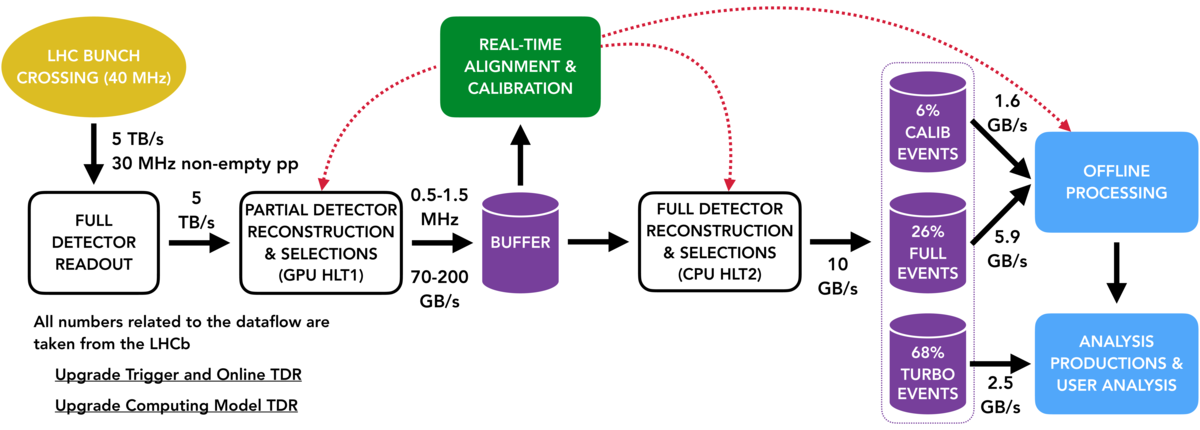
\includegraphics[width=\textwidth]{figures/hidef_RTA_dataflow_widescreen.png}
    \caption{Workflow of the Real Time Analysis paradigm, from the detector readout to analysis production}
    \label{fig:RTA}
\end{figure}

The trigger system now implements a two-stage full software solution, schematized in Figure~\ref{fig:RTA}:
\begin{itemize}
\item HLT$1$: the first stage, implemented on Graphics Processing Units (GPUs), operates on Event Builder (EB) nodes, reducing the data rate by a factor of 30-60.
\item HLT$2$: the second stage, running on Central Processing Units (CPUs) allows for detailed event reconstruction with quasi-offline precision~\cite{Gazzoni:2670650}.
\end{itemize}
Between HLT$1$ and HLT$2$, a buffer is implemented where the Alignment \& Calibration phase of the detector elements is performed.

The DAQ system~\cite{CERN-LHCC-2014-016} is composed of several sub-systems:
\begin{itemize}
\item Event Builder (EB)
\item Timing and Fast Control (TFC)
\item Event Filter Farm (EFF)
\item Experimental Control System (ECS)
\end{itemize}
In the following subsections, an overview of each subsystem is going to be presented. 

\subsection{Event Builder}
The data from all the sub-detectors in the underground area are transmitted to the surface through radiation-hard 300-meter-long optical fibers with zero-suppression, reducing unnecessary information before being transmitted. Each detector sends its data to a specific set of EB nodes. Within each EB node, custom PCIe boards (called PCIe40) equipped with FPGA chips process the incoming data, providing an interface between the front-end electronics and the other control systems, such as TFC and ECS). This preprocessing step is crucial, as it reduces the data load for subsequent stages. Each EB node processes a portion of the event data, requiring to exchange information with other EB nodes to assemble complete event information. This distributed approach reduces the amount of data any single node must process, ensuring efficiency and scalability. The EB nodes are interconnected through the Event Builder Network, which is designed to facilitate high-speed data exchange and event building.




\subsection{Timing and Fast Control}
The TFC system is responsible for distributing critical clock, timing, and trigger information to the front-end and readout systems. It synchronizes to the LHC master clock, ensuring precise timing across all components. The TFC provides global signals, including the \SI{40}{\mega\hertz} clock, synchronous commands to control event processing, calibration commands for detectors, and electronics configuration distribution from the ECS.

\subsection{Event Filter Farm}
The Event Filter Farm (EFF) hosts the hardware architectures for the high-level triggers (HLT). The HLT sequence comprises two stages: HLT$1$ and HLT$2$, separated by a disk buffer that holds events between stages while the detector is aligned and calibrated with offline precision.
\subsubsection{HLT$1$}
The HLT$1$ stage aims to reject events that do not contain particles of interest while retaining those that do. It uses a subset of the full offline charged particle reconstruction and implements inclusive single or two-track selections to determine the event's interest. HLT$1$ is entirely implemented on GPUs in the same servers hosting the Event Builder. The \textit{Allen} application, written in C++ with CUDA extensions, executes the following tasks~\cite{CERN-LHCC-2020-006}:
\begin{itemize}
\item Decoding raw input into the LHCb global coordinate system
\item Clustering detector hits
\item Pattern recognition to identify hit combinations associated with the same particle
\item Fitting track candidates using a Kalman Filter to estimate momentum and other parameters
\item Reconstructing primary and secondary vertices from fitted tracks
\item Making trigger decisions based on track parameters like impact parameter and momentum
\end{itemize}
The majority of tracks are created near the interaction point, and these are reconstructed as long tracks. However, some neutral long-lived particles, like $K^0_S$ and $\Lambda^0$, are reconstructed as downstream tracks because they decay outside the acceptance of the VELO detector. HLT$1$ focuses on long tracks, while HLT$2$ includes downstream tracks in its reconstruction sequence, allowing more comprehensive event analysis.
\subsubsection{Alignment and Calibration}\label{sec:alignment}
LHCb distinguishes between two phases~\cite{Dziurda:2640712}:
\begin{itemize}
\item Alignment focuses on correcting shifts and rotations in the detector's components, ensuring that the data obtained from these detectors are accurate. This process is applied to tracking detectors like VELO, UT, SciFi, and Muon systems, ensuring that their positioning aligns with the expected geometry.
\item Calibration involves fine-tuning the responses of various sub-detectors to ensure accurate measurements. This includes calibrating the RICH, ECAL, and HCAL.
\end{itemize}
Both processes are triggered at the beginning of each LHC fill, and they are fully integrated into the LHCb control system. 
\paragraph{Alignment}
Alignment at LHCb involves minimizing the chi-squared $\chi^2$ of all tracks with respect to alignment parameters $\alpha$, which account for translations and rotations of detector elements. The procedure employs the iterative Newton-Raphson method, where the first and second derivatives of $\chi^2$ with respect to 
 $\alpha$ are calculated to determine the optimal adjustments needed for alignment. The data for this alignment procedure comes from tracks obtained through a Kalman filter used in track reconstruction~\cite{HULSBERGEN2009471}, with the option to add vertex and mass constraints for increased precision.

The alignment process has two key components~\cite{Saur:20230E}:
\begin{itemize}
\item Analyzer: This part runs the track reconstruction, computes the $\chi^2$ derivatives, and saves them to binary files. It uses multi-threaded reconstruction based on 163 nodes, allowing for efficient data processing.
\item Iterator: This component collects the derivatives from the Analyzer, performs the minimization step, and checks for convergence. If there is a significant difference between the previous and new alignment constants, the updated constants are used in the HLT2 trigger, ensuring that subsequent data collection reflects the corrected alignment.
\end{itemize}
\paragraph{Calibration}
Calibration at LHCb involves ensuring that the detector responses are accurate and consistent. It typically includes:
\begin{itemize}
\item RICH Calibration: This involves calibrating the mirror positions and alignment to ensure accurate Cherenkov angle measurements.
\item Calorimeter Calibration: ECAL and HCAL calibration focuses on ensuring accurate energy measurements.
\end{itemize}
The calibration process leverages dedicated HLT1 trigger lines to select events suitable for calibration and alignment. These events are stored in a buffer until sufficient statistics are accumulated to run the calibration and alignment procedure. This buffering allows HLT2 reconstruction to use the most accurate and relevant alignment and calibration constants.
\subsubsection{HLT$2$}
While HLT$1$ focuses on long tracks, HLT$2$ conducts a full reconstruction, using information from tracking detectors and particle identification systems (RICHs, calorimeters, and muon chambers). It applies specialized cuts to select events of interest to LHCb.

\subsection{Experimental Control System}

The ECS~\cite{GranadoCardoso:2702137} oversees the entire LHCb experiment, from infrastructure to data acquisition. It is a distributed system based on the commercial SCADA system WinCC OA, and custom-developed components. The ECS features user interfaces, data archiving, alarm handling, and various device interfaces. Its tree-like control hierarchy, based on a Finite State Machine (FSM), allows commands to be propagated downstream and state information to be propagated upward. This structure provides centralized control and monitoring, ensuring efficient management of the LHCb experiment.



%Example of \autoref{alg:1} reference.

%\begin{algorithm}
%    \caption{Pseudocode}
%    \label{alg:1}
%    \begin{algorithmic}
%        \STATE $i\gets 10$
%        \IF {$i\geq 5$} 
%          \STATE $i\gets i-1$
%        \ELSE
%          \IF {$i\leq 3$}
%            \STATE $i\gets i+2$
%          \ENDIF
%        \ENDIF 
%    \end{algorithmic}
%\end{algorithm}